\documentclass[tikz,border=8pt]{standalone}
\usepackage[utf8]{inputenc}
\usepackage[OT4,plmath]{polski}
\usepackage{amsmath}
\begin{document}
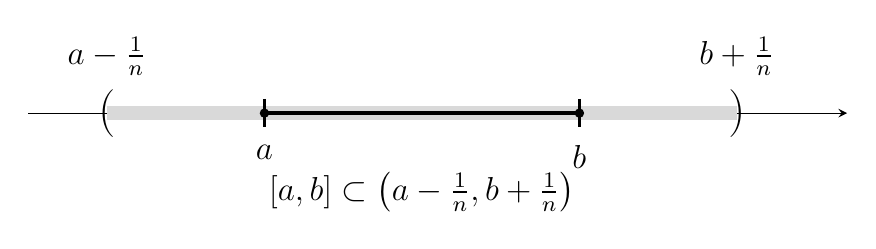
\begin{tikzpicture}[font=\large,>=stealth]
  \draw[->] (0,0)--(10.4,0);
  \draw[line width=5pt,black!15] (1,0)--(9,0);
  \draw[very thick] (3,0)--(7,0);
  \node[font=\LARGE] at (1,0) {$(\vphantom{b}$};
  \node[font=\LARGE] at (9,0) {$)\vphantom{b}$};
  \draw[thick] (3,.18)--(3,-.18) (7,.18)--(7,-.18);
  \fill (3,0) circle (1.7pt) (7,0) circle (1.7pt);
  \node[below=8pt] at (3,0) {$a$};
  \node[below=8pt] at (7,0) {$b$};
  \node[above=10pt] at (1,0) {$a-\frac1n$};
  \node[above=10pt] at (9,0) {$b+\frac1n$};
  \node at (5,-1) {$[a,b]\subset\left(a-\frac1n,b+\frac1n\right)$};
\end{tikzpicture}
\end{document}
